\documentclass[12pt,a4paper]{article}

\usepackage[a4paper,margin=1in]{geometry}
\usepackage[T1]{fontenc}
\usepackage[utf8]{inputenc}
\usepackage{lmodern}
\usepackage{setspace}
\usepackage{graphicx}
\usepackage{booktabs}
\usepackage{longtable}
\usepackage{array}
\usepackage{enumitem}
\usepackage{hyperref}
\usepackage{xcolor}
\usepackage{listings}
\usepackage{tikz}
\usepackage{float}
\usepackage{titlesec}
\usepackage{fancyhdr}

\usetikzlibrary{arrows.meta,positioning,shapes.geometric,fit,backgrounds}

\graphicspath{{screenshots/}}

\hypersetup{
    colorlinks=true,
    linkcolor=darkblue,
    urlcolor=darkblue,
    pdftitle={PLC Assignment 2 Report},
    pdfauthor={Kyal Sin Lin Lett, Wai Yan Aung, Aakriti Poudel}
}

\definecolor{codebg}{RGB}{247,247,247}
\definecolor{darkblue}{RGB}{20,54,96}
\definecolor{softgray}{RGB}{85,85,85}

\lstdefinestyle{plcstyle}{
    backgroundcolor=\color{codebg},
    basicstyle=\ttfamily\small,
    breaklines=true,
    frame=single,
    columns=fullflexible,
    keepspaces=true,
    showstringspaces=false
}

\lstset{style=plcstyle}

\setstretch{1.15}
\pagestyle{fancy}
\fancyhf{}
\fancyhead[L]{PLC Assignment 2}
\fancyhead[R]{Programming Language and Compiler}
\fancyfoot[C]{\thepage}

\titleformat{\section}{\large\bfseries\color{darkblue}}{\thesection}{0.75em}{}
\titleformat{\subsection}{\normalsize\bfseries\color{darkblue}}{\thesubsection}{0.75em}{}
\titleformat{\subsubsection}{\normalsize\bfseries}{\thesubsubsection}{0.75em}{}

\begin{document}

\begin{titlepage}
    \centering
    \vspace*{1.0cm}

    {\Huge\bfseries\color{darkblue}
    Programming Language Project\par}

    \vspace{0.5cm}

    {\Large\itshape\color{softgray}
    Design and Implementation of a Programming Language\par}

    \vspace{1.3cm}

    \vspace{0.3cm}

    {\large\color{softgray}
    Group:  Backus--Naur Form (BNF)\par}

    \vspace{2.0cm}

    {\Large\itshape\color{darkblue} Prepared by\par}

    \vspace{0.8cm}

    {\Large\color{darkblue}
    Kyal Sin Lin Lett \quad | \quad
    Wai Yan Aung \quad | \quad
    Aakriti Poudel\par}

    \vspace{1.8cm}

    {\Large\bfseries\color{darkblue}
    Course: Programming Language and Compiler\par}

    \vspace{1.6cm}

    {\Large\bfseries\color{darkblue}
    Submitted to\par}

    \vspace{0.3cm}

    {\Large\color{darkblue}
    Prof. Phan Min Dung\par}

    {\Large\color{darkblue}
    Mr. Akraradet Sinsamersuk\par}

    \vfill

    {\Large\bfseries\color{darkblue}
    Asian Institute of Technology\par}

    \vspace{0.2cm}

    {\Large\color{darkblue}
    FAST\par}

    \vspace{0.8cm}

    {\Large\color{softgray}
    May 2026\par}

\end{titlepage}

\tableofcontents
\newpage

\section{Abstract}
This report presents the design and implementation of a small statically typed programming language developed for the course \textit{Programming Language and Compiler}. The project provides a complete end-to-end language pipeline starting from source code input, proceeding through lexical analysis, parsing, abstract syntax tree construction, semantic/type checking, and finally execution through an interpreter runtime. The implementation is written in Python and uses the \texttt{SLY} toolkit for the lexer and parser and \texttt{PySide6} for the graphical user interface.

The language supports integer, floating-point, boolean, and string values; arithmetic and comparison expressions; assignment; conditional execution with \texttt{if} and \texttt{else}; iteration using \texttt{while}; function declaration and invocation; return statements; and a \texttt{print()} operation for user-visible output. The language also enforces static typing and static (lexical) binding. Variable types are inferred from first assignment and remain fixed afterward. Function parameter types and return types are inferred from the first valid call and subsequently enforced consistently. Name resolution follows lexical scoping rules, meaning a function can access its own local bindings and global bindings, but not the caller's local environment.

In addition to the language core, the project includes a desktop integrated development environment (IDE)-style interface that allows users to enter programs, run them, and inspect standard output or error messages. A comprehensive test suite validates the implementation at multiple levels, including lexer, parser, expression evaluation, statements, and full integration behavior. This report documents the language design, compiler/interpreter architecture, typing and binding algorithms, recursion readiness, testing strategy, current limitations, and possible future improvements.

\section{Introduction}
Programming language implementation is one of the clearest ways to combine theory with practice in compiler construction. A language project forces the developer to think carefully about syntax, semantics, runtime behavior, type systems, and error handling. Rather than only reading formal definitions of grammars, scope, or type checking, one must encode these ideas into real data structures and algorithms.

The goal of this project was to build a compact yet meaningful language that demonstrates core compiler concepts while still remaining understandable and testable within one course assignment. The project requirements asked for support for four basic types, static typing, arithmetic precedence, boolean expressions, assignment statements,if-then-else, while, function abstraction with value parameter passing, and a print function. Our implementation satisfies these requirements and further packages them into a small IDE-style graphical application.

Although the implementation ultimately executes programs through an interpreter rather than generating assembly or bytecode, it still follows the classic compiler structure. The system lexes raw source text, parses it into structured syntax, transforms it into an AST, performs a semantic/type checking pass, and only then executes the validated program. This separation is important because it mirrors how production language systems are structured and gives us a clean place to reason about typing, binding, and function behavior.

\subsection{Project Objectives}
The main objectives of PLC Assignment 2 are listed below.

\begin{enumerate}[leftmargin=1.2cm]
    \item Design a clear grammar for a small language with statements and expressions.
    \item Implement lexical analysis for reserved words, identifiers, literals, operators, and delimiters.
    \item Implement parsing rules that produce a structured AST rather than directly evaluating every construct during parsing.
    \item Enforce static typing and static binding using explicit semantic analysis.
    \item Support function abstraction, value parameter passing, and recursion.
    \item Provide a basic GUI so a user can edit and run programs interactively.
    \item Validate the system with automated tests and example programs.
\end{enumerate}

\subsection{Implemented Language Features}
The final integrated system supports the following language features:

\begin{itemize}[leftmargin=1.0cm]
    \item Primitive data types: \texttt{INT}, \texttt{FLOAT}, \texttt{BOOL}, and \texttt{STRING}
    \item Arithmetic expressions with precedence: \texttt{+}, \texttt{-}, \texttt{*}, \texttt{/}, unary minus
    \item Comparison expressions: \texttt{==}, \texttt{!=}, \texttt{<}, \texttt{<=}, \texttt{>}, \texttt{>=}
    \item Statements: assignment, \texttt{print}, \texttt{if}, \texttt{if-else}, \texttt{while}, \texttt{return}
    \item Function declarations and function calls
    \item Pass-by-value argument passing
    \item Static type inference and checking
    \item Static (lexical) scope resolution
    \item Recursion support
    \item Graphical editing and execution environment
\end{itemize}

\section{Language Specification}
\subsection{Lexical Elements}
The lexer identifies the lexical building blocks of the language. These include:

\begin{itemize}[leftmargin=1.0cm]
    \item Identifiers: user-defined variable and function names
    \item Integer literals: sequences of digits such as \texttt{42}
    \item Floating-point literals: values such as \texttt{3.14}
    \item Boolean literals: \texttt{true}, \texttt{false}
    \item String literals: text enclosed in double quotes
    \item Reserved words: \texttt{if}, \texttt{else}, \texttt{while}, \texttt{func}, \texttt{return}, \texttt{print}
    \item Operators: arithmetic and comparison operators
    \item Delimiters: parentheses, braces, commas, semicolons
\end{itemize}

The lexical layer is implemented using \texttt{SLY}'s lexer API, where each token is either declared with a regular expression or specialized through a token action function. This approach keeps the tokenization phase explicit and deterministic.

\subsection{Grammar}
The final grammar used by the integrated system is shown below.

\begin{lstlisting}
<program>   ::= <stmts>

<stmts>     ::= <stmts> <stmt> | epsilon

<stmt>      ::= NAME ASSIGN <expr> SEMI
              | IF LPAREN <expr> RPAREN <block>
              | IF LPAREN <expr> RPAREN <block> ELSE <block>
              | WHILE LPAREN <expr> RPAREN <block>
              | PRINT LPAREN <expr> RPAREN SEMI
              | FUNC NAME LPAREN <params> RPAREN <block>
              | RETURN <expr> SEMI
              | <expr> SEMI

<block>     ::= LBRACE <stmts> RBRACE

<params>    ::= <params> COMMA NAME | NAME | epsilon

<expr>      ::= <expr> PLUS <expr>
              | <expr> MINUS <expr>
              | <expr> TIMES <expr>
              | <expr> DIVIDE <expr>
              | <expr> EQUAL <expr>
              | <expr> NOT_EQUAL <expr>
              | <expr> LESS <expr>
              | <expr> LESS_EQUAL <expr>
              | <expr> GREATER <expr>
              | <expr> GREATER_EQUAL <expr>
              | MINUS <expr>
              | LPAREN <expr> RPAREN
              | NAME LPAREN <args> RPAREN
              | NAME
              | NUMBER | FLOAT | TRUE | FALSE | STRING

<args>      ::= <args> COMMA <expr> | <expr> | epsilon
\end{lstlisting}

\subsection{Operator Precedence}
The parser resolves expressions using the precedence table below.

\begin{table}[H]
\centering
\begin{tabular}{lll}
\toprule
Level & Operators & Associativity \\
\midrule
1 & \texttt{== != < <= > >=} & left \\
2 & \texttt{+ -} & left \\
3 & \texttt{* /} & left \\
4 & unary \texttt{-} & right \\
\bottomrule
\end{tabular}
\caption{Operator precedence in the PLC language}
\end{table}

\section{System Architecture}
The project follows a staged language-processing pipeline. Even though the runtime execution is interpreted, the structure still resembles a compiler front-end followed by a semantic analysis phase and an execution engine.

\subsection{High-Level Processing Flow}

\begin{figure}[H]
\centering
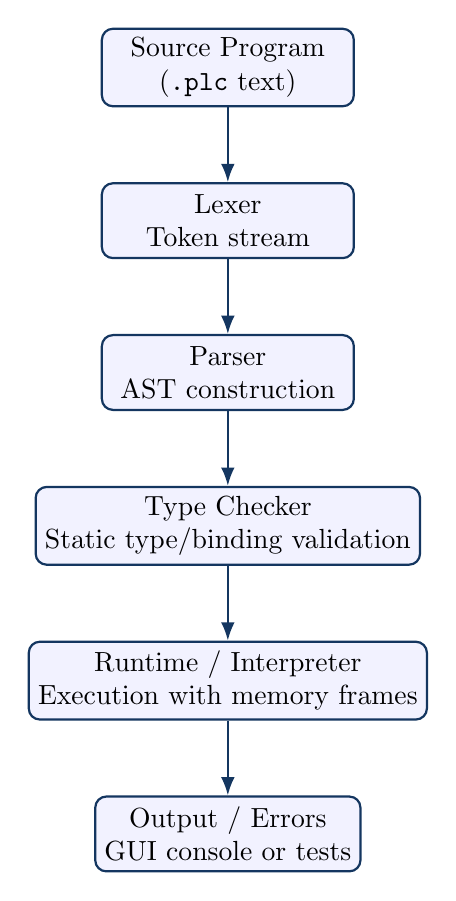
\begin{tikzpicture}[
    node distance=0.95cm,
    box/.style={draw=darkblue, rounded corners, thick, minimum width=3.2cm, minimum height=0.95cm, align=center, fill=blue!5},
    line/.style={-Latex, thick, darkblue}
]
\node[box] (src) {Source Program\\(\texttt{.plc} text)};
\node[box, below=of src] (lexer) {Lexer\\Token stream};
\node[box, below=of lexer] (parser) {Parser\\AST construction};
\node[box, below=of parser] (typecheck) {Type Checker\\Static type/binding validation};
\node[box, below=of typecheck] (runtime) {Runtime / Interpreter\\Execution with memory frames};
\node[box, below=of runtime] (output) {Output / Errors\\GUI console or tests};

\draw[line] (src) -- (lexer);
\draw[line] (lexer) -- (parser);
\draw[line] (parser) -- (typecheck);
\draw[line] (typecheck) -- (runtime);
\draw[line] (runtime) -- (output);
\end{tikzpicture}
\caption{Overall system pipeline}
\end{figure}

\subsection{Compiler Components Diagram}

\begin{figure}[H]
\centering
\resizebox{\textwidth}{!}{%
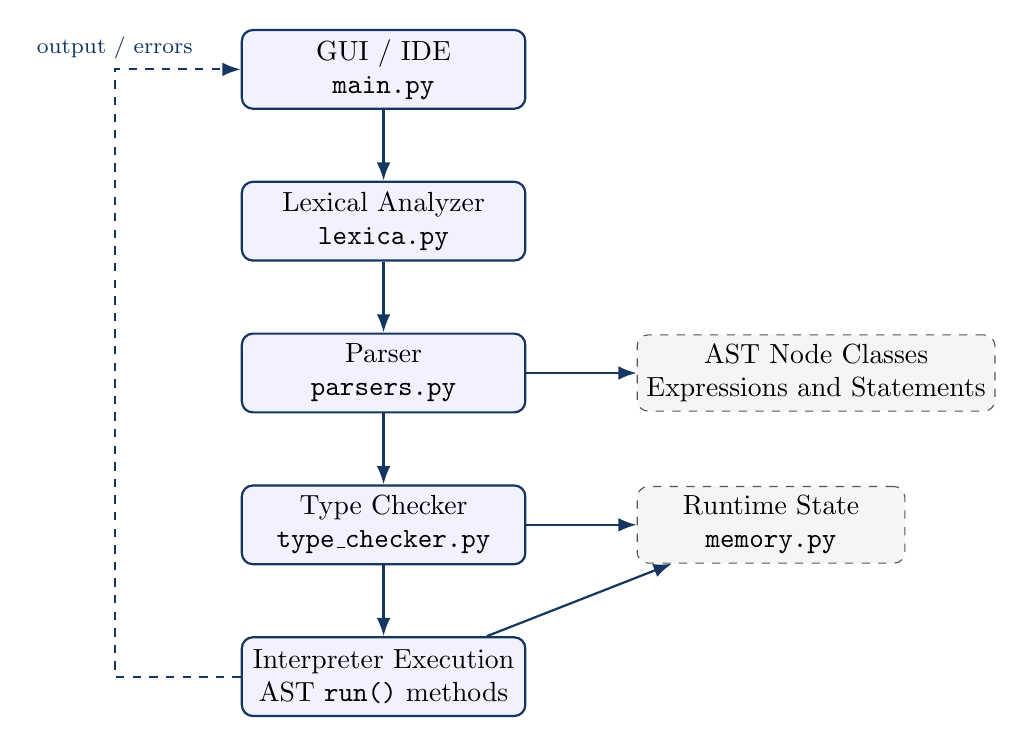
\begin{tikzpicture}[
    node distance=0.9cm and 1.4cm,
    comp/.style={draw=darkblue, rounded corners, thick, minimum width=3.6cm, minimum height=1.0cm, align=center, fill=blue!5},
    data/.style={draw=softgray, rounded corners, dashed, minimum width=3.4cm, minimum height=0.9cm, align=center, fill=gray!8},
    arr/.style={-Latex, thick, darkblue},
    feedback/.style={-Latex, thick, darkblue, dashed}
]
\node[comp] (gui) {GUI / IDE\\\texttt{main.py}};
\node[comp, below=of gui] (lex) {Lexical Analyzer\\\texttt{lexica.py}};
\node[comp, below=of lex] (parse) {Parser\\\texttt{parsers.py}};
\node[data, right=of parse] (ast) {AST Node Classes\\Expressions and Statements};
\node[comp, below=of parse] (tc) {Type Checker\\\texttt{type\_checker.py}};
\node[data, right=of tc] (mem) {Runtime State\\\texttt{memory.py}};
\node[comp, below=of tc] (exec) {Interpreter Execution\\AST \texttt{run()} methods};

\draw[arr] (gui) -- (lex);
\draw[arr] (lex) -- (parse);
\draw[arr] (parse) -- (tc);
\draw[arr] (parse) -- (ast);
\draw[arr] (tc) -- (exec);
\draw[arr] (tc) -- (mem);
\draw[arr] (exec) -- (mem);
\draw[feedback] (exec.west) -- ++(-1.6,0) |- (gui.west)
    node[midway, above, sloped, font=\footnotesize, color=darkblue] {output / errors};
\end{tikzpicture}%
}
\caption{Component-level architecture of the PLC system. Solid arrows show the forward processing pipeline; the dashed arrow shows the runtime returning output and error messages back to the GUI.}
\end{figure}

\subsection{Module Responsibilities}
\begin{longtable}{>{\raggedright\arraybackslash}p{3.2cm} >{\raggedright\arraybackslash}p{10.5cm}}
\toprule
\textbf{Module} & \textbf{Responsibility} \\
\midrule
\endfirsthead
\toprule
\textbf{Module} & \textbf{Responsibility} \\
\midrule
\endhead
\texttt{lexica.py} & Converts program text into tokens such as identifiers, literals, reserved words, operators, and delimiters. \\
\texttt{parsers.py} & Defines grammar rules and constructs AST nodes from the token stream. \\
\texttt{ast/statement.py} & Contains AST classes for statements and expressions in the integrated branch, plus runtime execution behavior. \\
\texttt{type\_checker.py} & Performs semantic checking and enforces typing and binding rules before program execution. \\
\texttt{memory.py} & Maintains runtime variable frames, function definitions, and output buffer. \\
\texttt{main.py} & Provides the GUI, code editor, run button, output console, and error console. \\
\texttt{tests/} & Verifies system behavior at lexer, parser, expression, statement, and integration levels. \\
\texttt{examples/} & Contains sample PLC programs demonstrating language features. \\
\bottomrule
\end{longtable}

\section{Lexical Analysis}
Lexical analysis is the first operational stage of the system. The source program is scanned from left to right and segmented into tokens. The implementation uses regular expressions to identify tokens and direct token-to-keyword mapping for reserved words. This design is well suited to a small educational language because the token set is compact and each token category is easy to specify declaratively.

The lexer supports both symbolic tokens and keyword tokens. For instance, a character sequence that matches the general identifier pattern may later be reclassified as \texttt{IF}, \texttt{WHILE}, or \texttt{FUNC} if it matches a reserved word. This is a standard and effective design pattern in compiler front-ends.

The lexer also handles value conversion for numeric and string literals. Integer tokens are converted into Python \texttt{int}, floating tokens into Python \texttt{float}, and string tokens are stored without their surrounding quotes. Because the conversion happens during lexing, later phases can work with already-normalized literal values.

\section{Parsing and AST Construction}
\subsection{Why an AST-Based Design Was Chosen}
The project does not directly execute syntax rules during parsing. Instead, it builds an abstract syntax tree and then processes that tree in later phases. This decision is especially important for statements and function semantics. Constructs such as \texttt{if}, \texttt{while}, and \texttt{return} require deferred control flow. They cannot be evaluated correctly if reduced immediately in the parser without a tree structure.

An AST also improves modularity. The parser becomes responsible only for structure, while semantics are handled in dedicated AST methods and the type checker. This separation was especially useful in our project because different team members worked on expressions, statements, GUI integration, and test coverage.

\subsection{Expression Nodes}
The AST includes nodes for:

\begin{itemize}[leftmargin=1.0cm]
    \item integer literals
    \item floating-point literals
    \item boolean literals
    \item string literals
    \item variable references
    \item arithmetic expressions
    \item comparison expressions
    \item unary negation
    \item function-call expressions
\end{itemize}

Each expression node stores both a runtime value slot and a \texttt{DataType} slot. This dual representation is important. The value is used during execution, while the type is used both during semantic analysis and for runtime sanity checks.

\subsection{Statement Nodes}
The AST includes nodes for:

\begin{itemize}[leftmargin=1.0cm]
    \item assignment statements
    \item print statements
    \item block statements
    \item if statements
    \item while statements
    \item function declarations
    \item return statements
    \item bare expression statements
\end{itemize}

Blocks are represented explicitly as lists of statements, allowing nested control flow and function bodies to be processed recursively. Return statements use a special return-signal mechanism to unwind execution out of the current function body.

\section{Type System}
\subsection{Overview}
The language is statically typed, but it does not require explicit type declarations. Instead, types are inferred from the first valid assignment or first valid function call. This design gives the language some syntactic simplicity while still enforcing strong type consistency.

The primitive types are:
\begin{itemize}[leftmargin=1.0cm]
    \item \texttt{INT}
    \item \texttt{FLOAT}
    \item \texttt{BOOL}
    \item \texttt{STRING}
    \item \texttt{VOID} for functions that do not return a value
\end{itemize}

\subsection{Static Type Rules}
The system enforces the following static rules:

\begin{enumerate}[leftmargin=1.2cm]
    \item A variable's type is fixed by its first assignment.
    \item A later assignment to the same variable must use the same type.
    \item Arithmetic operands must have the same type and must be numeric (\texttt{INT} or \texttt{FLOAT}).
    \item Comparisons must compare same-typed numeric operands.
    \item \texttt{if} and \texttt{while} conditions must evaluate to \texttt{BOOL}.
    \item The number of call arguments must match the function parameter count.
    \item Function parameter types are inferred from the first successful call and must remain consistent.
    \item Function return type is inferred from observed return statements and must remain consistent.
\end{enumerate}

\subsection{Translation Scheme for Type Checking}
The static rules above can be presented formally as a translation scheme in the style of attribute grammars. Each production carries a semantic action (in braces) that synthesizes a \texttt{type} attribute on the left-hand-side construct from the attributes of its sub-components, possibly with side effects on a global environment.

We adopt the following conventions:
\begin{itemize}[leftmargin=1.0cm]
    \item $\mathit{env}$ is the variable environment, a partial map from names to types. \texttt{env(id)} reads the current type binding for \texttt{id}; \texttt{env(id) := T} installs a new binding.
    \item $F$ ranges over functions in the function table. $F.\mathit{params}$ is its parameter-type vector and $F.\mathit{ret}$ is its return type. Both start unbound and are filled in on the first call.
    \item Well-typed statements yield $S.\mathit{type} = \mathtt{void}$; ill-typed constructs yield $\mathtt{type\_error}$ which propagates upward.
    \item A successful semantic action may also have side effects (binding a name, registering a function, or checking a function body); these are written in the action body.
\end{itemize}

\begin{figure}[H]
\centering
\resizebox{\textwidth}{!}{%
\renewcommand{\arraystretch}{1.4}
\begin{tabular}{@{}l@{\hspace{1.2em}}l@{}}
$S \rightarrow id := E$ &
$\{$ \texttt{if id $\notin$ env then env(id) := E.type; S.type := void} \\
& \hspace{1.0em}\texttt{else if env(id) = E.type then S.type := void} \\
& \hspace{1.0em}\texttt{else S.type := type\_error} $\}$ \\

$S \rightarrow \mathbf{if}\ E\ \mathbf{then}\ S_1$ &
$\{$ \texttt{S.type := if E.type = boolean and $S_1$.type = void} \\
& \hspace{1.0em}\texttt{then void else type\_error} $\}$ \\

$S \rightarrow \mathbf{if}\ E\ \mathbf{then}\ S_1\ \mathbf{else}\ S_2$ &
$\{$ \texttt{S.type := if E.type = boolean and} \\
& \hspace{1.0em}\texttt{$S_1$.type = void and $S_2$.type = void} \\
& \hspace{1.0em}\texttt{then void else type\_error} $\}$ \\

$S \rightarrow \mathbf{while}\ E\ \mathbf{do}\ S_1$ &
$\{$ \texttt{S.type := if E.type = boolean and $S_1$.type = void} \\
& \hspace{1.0em}\texttt{then void else type\_error} $\}$ \\

$S \rightarrow S_1\ ;\ S_2$ &
$\{$ \texttt{S.type := if $S_1$.type = void and $S_2$.type = void} \\
& \hspace{1.0em}\texttt{then void else type\_error} $\}$ \\

$S \rightarrow \mathbf{print}\ E$ &
$\{$ \texttt{S.type := if E.type $\in$ \{int, float, bool, string\}} \\
& \hspace{1.0em}\texttt{then void else type\_error} $\}$ \\

$S \rightarrow \mathbf{return}\ E$ &
$\{$ \texttt{let F = enclosing function;} \\
& \hspace{1.0em}\texttt{if F.ret unbound then F.ret := E.type; S.type := void} \\
& \hspace{1.0em}\texttt{else if F.ret = E.type then S.type := void} \\
& \hspace{1.0em}\texttt{else S.type := type\_error} $\}$ \\

$S \rightarrow \mathbf{func}\ id(p_1,\ldots,p_n)\ S_1$ &
$\{$ \texttt{register function id with parameters $p_1,\ldots,p_n$} \\
& \hspace{1.0em}\texttt{and body $S_1$ in the function table;} \\
& \hspace{1.0em}\texttt{S.type := void} $\}$ \\

$S \rightarrow E$ &
$\{$ \texttt{S.type := if E.type $\neq$ type\_error} \\
& \hspace{1.0em}\texttt{then void else type\_error} $\}$ \\
\end{tabular}%
}
\caption{Translation scheme for checking the type of statements}
\end{figure}

\begin{figure}[H]
\centering
\resizebox{\textwidth}{!}{%
\renewcommand{\arraystretch}{1.4}
\begin{tabular}{@{}l@{\hspace{1.2em}}l@{}}
$E \rightarrow E_1\ \mathit{op}\ E_2$ &
$\{$ \texttt{E.type := if $E_1$.type = $E_2$.type and} \\
\textit{(op $\in$ \{+, -, *\})} & \hspace{1.0em}\texttt{$E_1$.type $\in$ \{int, float\}} \\
& \hspace{1.0em}\texttt{then $E_1$.type else type\_error} $\}$ \\

$E \rightarrow E_1\ /\ E_2$ &
$\{$ \texttt{E.type := if $E_1$.type = $E_2$.type and} \\
& \hspace{1.0em}\texttt{$E_1$.type $\in$ \{int, float\}} \\
& \hspace{1.0em}\texttt{then float else type\_error} $\}$ \\

$E \rightarrow E_1\ \mathit{relop}\ E_2$ &
$\{$ \texttt{E.type := if $E_1$.type = $E_2$.type and} \\
& \hspace{1.0em}\texttt{$E_1$.type $\in$ \{int, float\}} \\
& \hspace{1.0em}\texttt{then boolean else type\_error} $\}$ \\

$E \rightarrow -\,E_1$ &
$\{$ \texttt{E.type := if $E_1$.type $\in$ \{int, float\}} \\
& \hspace{1.0em}\texttt{then $E_1$.type else type\_error} $\}$ \\

$E \rightarrow id(a_1,\ldots,a_n)$ &
$\{$ \texttt{let F = lookup(id);} \\
& \hspace{1.0em}\texttt{if F undefined or arity(F) $\neq$ n} \\
& \hspace{2.0em}\texttt{then E.type := type\_error} \\
& \hspace{1.0em}\texttt{else if F.params unbound then} \\
& \hspace{2.0em}\texttt{F.params := ($a_1$.type,\ldots,$a_n$.type);} \\
& \hspace{2.0em}\texttt{check body of F; E.type := F.ret} \\
& \hspace{1.0em}\texttt{else if F.params = ($a_1$.type,\ldots,$a_n$.type)} \\
& \hspace{2.0em}\texttt{then E.type := F.ret} \\
& \hspace{1.0em}\texttt{else E.type := type\_error} $\}$ \\

$E \rightarrow id$ &
$\{$ \texttt{E.type := if id $\in$ env then env(id) else type\_error} $\}$ \\

$E \rightarrow \mathit{int\_lit}$ & $\{$ \texttt{E.type := int} $\}$ \\
$E \rightarrow \mathit{float\_lit}$ & $\{$ \texttt{E.type := float} $\}$ \\
$E \rightarrow \mathit{bool\_lit}$ & $\{$ \texttt{E.type := boolean} $\}$ \\
$E \rightarrow \mathit{str\_lit}$ & $\{$ \texttt{E.type := string} $\}$ \\
\end{tabular}%
}
\caption{Translation scheme for checking the type of expressions}
\end{figure}

Several design decisions are visible directly in the scheme. The assignment rule allows the first occurrence of a name to install a new binding, while a later occurrence must agree with the previously installed type --- this is what realizes \emph{static variable binding}. The division rule produces \texttt{float} regardless of whether the operands were both \texttt{int}, so the result type is determined statically from the operator, not from the runtime value. The \texttt{return} rule both reads and writes $F.\mathit{ret}$, so the first return statement encountered in a function body fixes the function's return type and every subsequent return must match it. The function-call rule similarly fixes $F.\mathit{params}$ on the first call, after which every later call is checked against the locked signature. Function bodies are checked lazily on the first call, when their parameter types are known.

\subsection{Type Checking Algorithm}
The type checker performs a full walk over the AST before execution. It can be summarized as follows:

\begin{enumerate}[leftmargin=1.2cm]
    \item Register all top-level function names.
    \item Traverse statements in order.
    \item For each assignment, infer the expression type and record or validate the variable type.
    \item For each condition, infer the expression type and require \texttt{BOOL}.
    \item For each function call, infer the argument types, validate arity, bind parameter types, and check the function body if needed.
    \item For recursive functions, temporarily track functions in progress so recursive calls can terminate semantic analysis without infinite recursion.
\end{enumerate}

This algorithm allows the project to behave like a statically typed interpreted language. That is, typing errors are detected before any AST execution occurs.

\subsection{Division Rule}
One notable design decision is that division always returns \texttt{FLOAT}, even when both operands are integers. For example:

\begin{lstlisting}
a = 10;
b = 2;
c = a / b;
\end{lstlisting}

The variable \texttt{c} will have type \texttt{FLOAT}. This rule was chosen to keep division semantics simple and unambiguous.

\section{Binding and Scope}
\subsection{Static Binding}
The language uses static (lexical) binding. This means that the meaning of a variable name is determined by the program structure rather than by the runtime call path. A function can access:

\begin{itemize}[leftmargin=1.0cm]
    \item variables in its own local frame
    \item variables in the global frame
\end{itemize}

It cannot access a caller's local frame. This is important because it prevents accidental dynamic scope behavior and keeps function meaning stable regardless of who calls the function.

\subsection{Memory Model}
The runtime environment uses a frame stack. The memory object stores:

\begin{itemize}[leftmargin=1.0cm]
    \item a global frame
    \item zero or more function-local frames
    \item a function table
    \item an output buffer
\end{itemize}

On each function call, a new local frame is pushed. On function return, the frame is popped. Variable lookup checks the current frame first and then the global frame. This realizes static binding in a simple and robust way.

\subsection{Illustration of Static Scope}
The sample program below demonstrates lexical scope:

\begin{lstlisting}
x = 1;

func inner() {
    print(x);
}

func outer() {
    x = 99;
    inner();
}
\end{lstlisting}

When \texttt{outer()} calls \texttt{inner()}, the function \texttt{inner()} prints the global \texttt{x}, not the local \texttt{x} in \texttt{outer()}. This proves that the implementation does not use dynamic binding.

\section{Functions, Parameter Passing, and Recursion}
\subsection{Function Abstraction}
Functions are declared using the keyword \texttt{func}. A function definition consists of:

\begin{itemize}[leftmargin=1.0cm]
    \item a function name
    \item a parameter list
    \item a block body
\end{itemize}

Example:
\begin{lstlisting}
func add(a, b) {
    return a + b;
}
\end{lstlisting}

\subsection{Parameter Passing}
The language uses \textbf{pass by value}. At call time:

\begin{enumerate}[leftmargin=1.2cm]
    \item argument expressions are evaluated,
    \item their values are copied into a fresh function-local frame,
    \item parameter names are bound to those copied values.
\end{enumerate}

Therefore, changing a parameter inside the function does not mutate the caller's variable binding.

\subsection{Recursion Readiness}
The integrated implementation is recursion-ready, both semantically and at runtime.

\paragraph{Runtime support.}
Runtime recursion works because each call pushes a new frame onto the memory stack. Recursive calls therefore do not overwrite each other's local variables.

\paragraph{Type-checking support.}
The type checker explicitly tracks functions currently being checked using an \texttt{in\_progress} set. When a recursive call is encountered inside the same function body, the checker avoids infinite recursion by reusing the partial function signature already inferred so far. This is a crucial detail: without it, recursive programs such as factorial or Fibonacci would either crash the type checker or never finish analysis.

\subsection{Example: Recursive Factorial}
\begin{lstlisting}
func factorial(n) {
    if (n < 2) {
        return 1;
    }
    return n * factorial(n - 1);
}

print(factorial(5));
\end{lstlisting}

This program is included in the project examples and demonstrates both recursion and static typing over recursive return values.

\section{GUI and User Interaction}
The project provides a graphical IDE-style application implemented using \texttt{PySide6}. The GUI is not merely decorative; it is an important usability layer that allows the language to be demonstrated interactively.

\subsection{GUI Components}
The interface includes:

\begin{itemize}[leftmargin=1.0cm]
    \item a code editor for writing PLC programs,
    \item syntax highlighting,
    \item a \texttt{Run} button,
    \item a \texttt{Clear} button,
    \item file open/save support,
    \item a program output panel,
    \item an error message panel.
\end{itemize}

\subsection{Execution Sequence from the GUI}
When the user presses \texttt{Run}, the system performs the following:

\begin{enumerate}[leftmargin=1.2cm]
    \item clear previous output and error messages,
    \item lex and parse the source text,
    \item if parsing fails, report syntax diagnostics,
    \item run the type checker on the AST,
    \item if typing succeeds, execute the AST,
    \item collect \texttt{print()} output from the runtime memory object,
    \item display final output or errors in the interface.
\end{enumerate}

This flow ensures that malformed or ill-typed programs do not proceed to execution.

\subsection{IDE in Action}
The two screenshots below illustrate the IDE's two output channels --- the program output panel for successful runs and the error panel for failures detected before or during execution.

\begin{figure}[H]
\centering
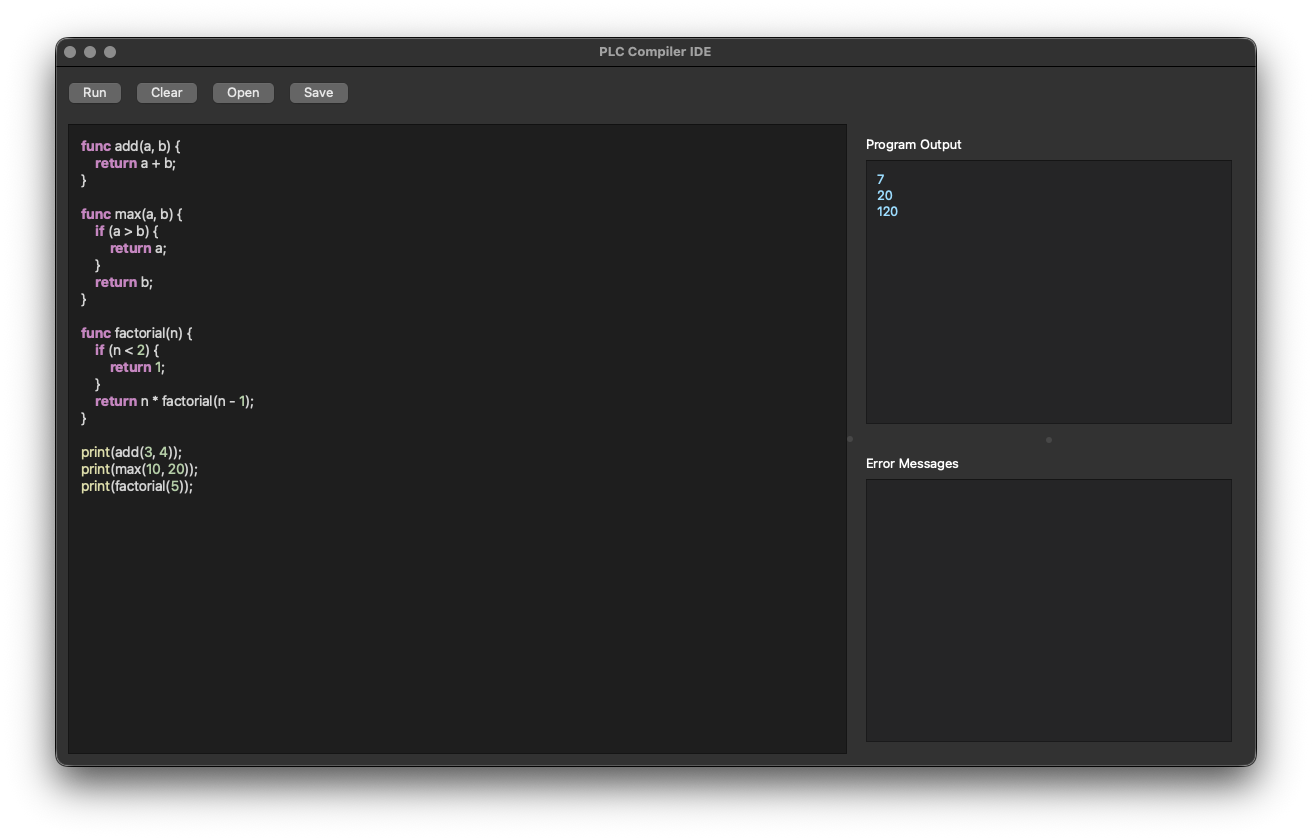
\includegraphics[width=0.92\textwidth]{happy}
\caption{Happy path: a program defining \texttt{add}, \texttt{max}, and a recursive \texttt{factorial} runs successfully. The output panel shows \texttt{7}, \texttt{20}, and \texttt{120} from \texttt{add(3,4)}, \texttt{max(10,20)}, and \texttt{factorial(5)} respectively. Syntax highlighting distinguishes keywords, function names, numeric literals, and string literals.}
\end{figure}

\begin{figure}[H]
\centering
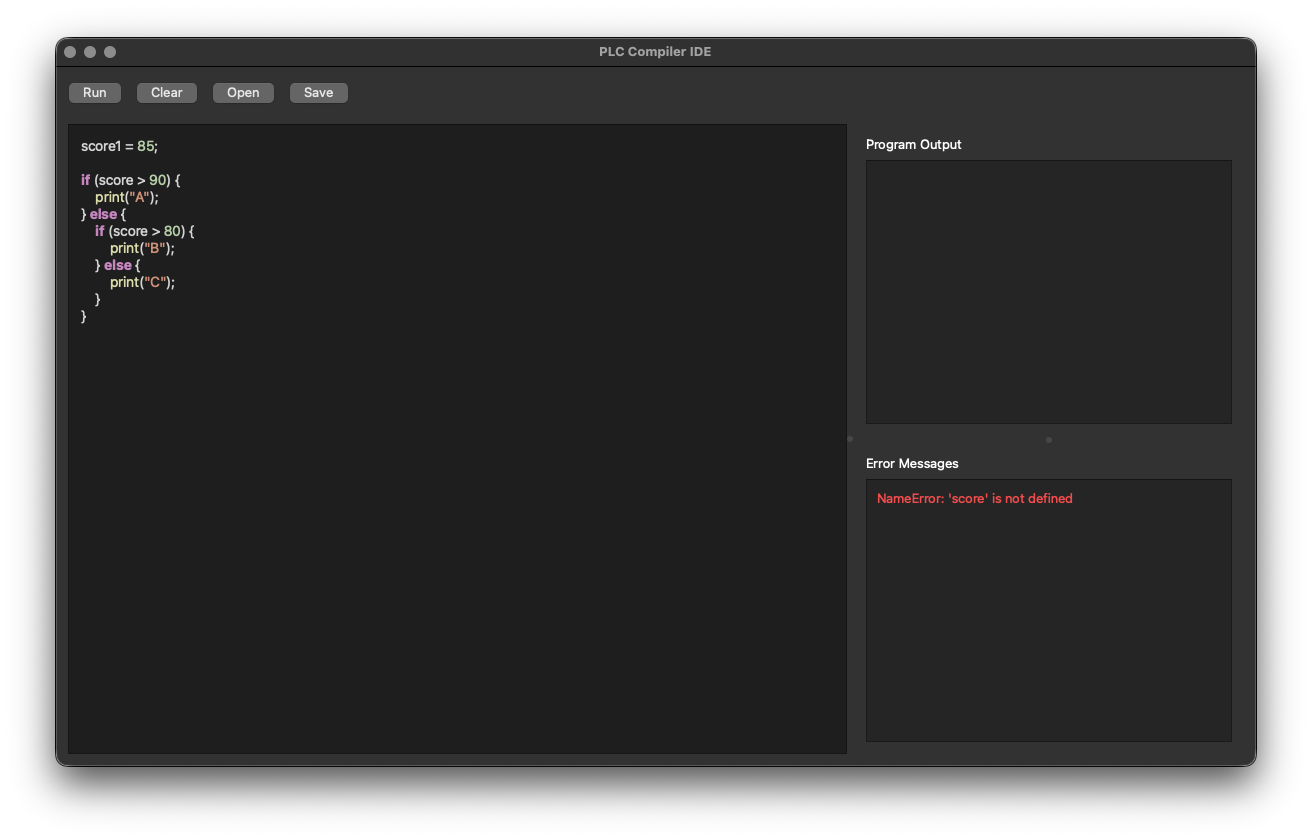
\includegraphics[width=0.92\textwidth]{sad}
\caption{Sad path: an \texttt{if-else} program references the variable \texttt{score}, but the assignment statement above mistakenly writes \texttt{score1 = 85;}. The type checker catches the use of an undeclared name before any branch executes and routes \texttt{NameError: 'score' is not defined} to the error console while the program output panel stays empty.}
\end{figure}

The two screenshots together demonstrate the design choice that motivated the dedicated type-checking pass: errors are reported to the user without any partial execution side effects, and the success and failure channels are visually separated rather than interleaved into a single console.

\section{Testing and Validation}
\subsection{Testing Strategy}
The project includes automated tests at multiple levels:

\begin{itemize}[leftmargin=1.0cm]
    \item lexer tests,
    \item parser tests,
    \item expression tests,
    \item statement tests,
    \item integration tests,
    \item example programs for manual demonstration.
\end{itemize}

This layered testing strategy is important because a language system can fail at many different points. Some bugs are lexical, some are grammatical, some are semantic, and some appear only during full execution.

\subsection{Covered Scenarios}
The test suite validates:

\begin{itemize}[leftmargin=1.0cm]
    \item token recognition for all major token classes,
    \item arithmetic precedence,
    \item correct typing of expressions,
    \item valid and invalid comparisons,
    \item assignment consistency,
    \item branch selection in \texttt{if-else},
    \item loop execution in \texttt{while},
    \item function invocation and return,
    \item static binding behavior,
    \item pass-by-value behavior,
    \item recursive execution,
    \item parser/type checker/runtime integration.
\end{itemize}

\subsection{Representative Example Programs}
The repository contains curated example files:

\begin{itemize}[leftmargin=1.0cm]
    \item \texttt{01\_types.plc}
    \item \texttt{02\_arithmetic.plc}
    \item \texttt{03\_if\_else.plc}
    \item \texttt{04\_while.plc}
    \item \texttt{05\_functions.plc}
    \item \texttt{06\_static\_type\_binding.plc}
    \item \texttt{07\_static\_scope\_binding.plc}
    \item \texttt{08\_pass\_by\_value.plc}
    \item \texttt{fibo.plc}
\end{itemize}

These example programs serve two purposes: they function as executable demonstrations during presentation, and they make the language semantics concrete for readers.

\section{Design Decisions and Rationale}
\subsection{Why Static Typing Was Chosen}
Static typing provides earlier error detection and makes program behavior more predictable. In an educational compiler project, it also creates a natural place to discuss semantic analysis, symbol tracking, and typing algorithms.

\subsection{Why Static Binding Was Chosen}
Static binding is easier to reason about and matches the intended semantics of most modern structured languages. It also highlights the distinction between lexical structure and runtime call behavior, which is a key topic in programming language theory.

\subsection{Why AST Execution Was Preferred over Direct Parser Evaluation}
Direct parser evaluation is suitable for calculators, but it becomes restrictive once control-flow statements and functions are introduced. AST execution gives much better separation of syntax and semantics and makes testing significantly easier.

\section{Current Limitations}
Although the system is complete with respect to the assignment requirements, several limitations remain:

\begin{itemize}[leftmargin=1.0cm]
    \item Explicit type annotations are not supported.
    \item Comparisons are restricted to numeric operands.
    \item There is no bytecode generation or machine-code compilation; execution is interpreted.
    \item Error reporting could still be improved with richer source locations.
    \item The parser currently reports shift/reduce conflicts internally, even though the integrated tests pass.
    \item The current environment-dependent GUI launch process may require specific Qt plugin availability.
\end{itemize}

\section{Possible Future Work}
Future extensions could include:

\begin{itemize}[leftmargin=1.0cm]
    \item explicit type declarations,
    \item arrays or lists,
    \item logical operators such as \texttt{and}, \texttt{or}, and \texttt{not},
    \item better error spans and highlighted source locations,
    \item bytecode generation,
    \item a more formal symbol table abstraction separate from the runtime memory object,
    \item optimization passes,
    \item a richer standard library.
\end{itemize}

\section{Conclusion}
PLC Assignment 2 demonstrates that a compact language can still illustrate many of the essential ideas of programming language implementation. The project includes formal grammar design, lexical analysis, parsing, AST construction, semantic analysis, static typing, static binding, function abstraction, pass-by-value semantics, recursion support, runtime execution, automated testing, and a GUI front-end.

The resulting system is not merely a calculator or a minimal parser. It is a structured educational language implementation whose components map directly to the core concepts taught in compiler and programming language courses. Static typing and lexical binding were especially important because they required us to build a semantic analysis phase rather than rely only on runtime evaluation. The final test suite and example programs show that the implementation behaves consistently and is ready for demonstration and academic submission.

\appendix
\section{Appendix: Example PLC Program}
\begin{lstlisting}
func factorial(n) {
    if (n < 2) {
        return 1;
    }
    return n * factorial(n - 1);
}

x = factorial(5);
print(x);
\end{lstlisting}

\section{Appendix: Summary of Core Semantic Rules}
\begin{itemize}[leftmargin=1.0cm]
    \item First assignment determines variable type.
    \item Reassignment with a new type is illegal.
    \item Arithmetic works only on same-typed numeric values.
    \item Comparison works only on same-typed numeric values.
    \item Conditions must be boolean.
    \item Functions are defined globally.
    \item Functions use pass by value.
    \item Functions use lexical scope.
    \item Recursive calls are supported by both runtime frames and semantic analysis.
\end{itemize}

\end{document}
